\section{Przygotowanie gramatyki kształtu twarzy}
W tym rozdziale przedstawiony jest opis przeprowadzonej analizy struktury
głowy oraz dyskusja o tym, jak taką strukturę zamodelować przy użyciu
gramatyki kształtu.
Przed przystąpieniem do dalszej pracy, musiała zostać podjęta decyzja co
do poziomu szczegółowości wirtualnego odpowiednika głowy. Z założenia gramatyka
nie ma ograniczeń, więc nic nie stoi na przeszkodzie, aby zbudować model zawierający
wszystkie najbardziej elementarne części głowy. Jednak z uwagi na charakter
tej pracy oraz pożądany efekt docelowy zostaną pominięte wszystkie elementy
wewnętrzne. Najistotniejsze są części bezpośrednio tworzące zewnętrzną
strukturę. Warto jednak zaznaczyć, że jeżeli zaszłaby taka potrzeba to można
zamodelować wewnętrzną strukturę głowy i sterując parametrami obserwować wpływ
poszczególnych części na siebie. Wszystko zależy od złożoności gramatyki.
Na ilustracji~\ref{wiola_jpg} zaprezentowana jest przykładowa głowa
w różnych rzutach wraz z liniami na wybranych charakterystycznych poziomach.
Kolejne linie (od góry do dołu) oznaczają: czubek głowy, poziom górnej oraz
dolnej granicy oczu, koniec nosa, górną oraz dolną granicę warg i podbródek.

\begin{figure}[h!]
\centering
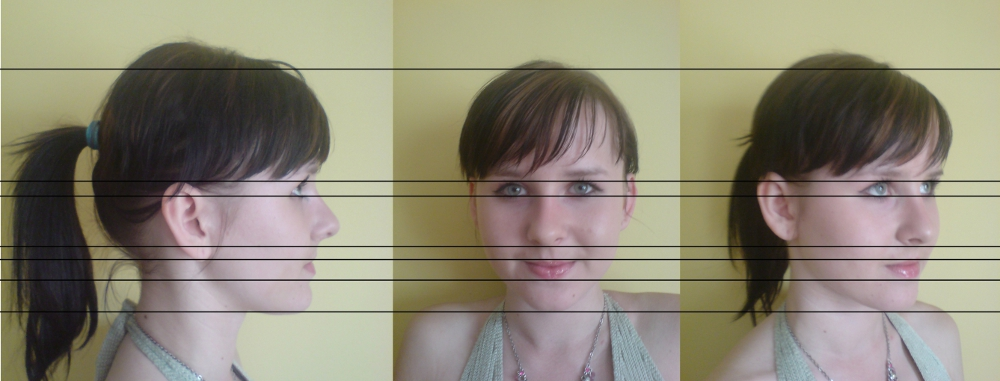
\includegraphics[width=14cm]{images/wiola.jpg}
\caption{Twarz w różnych rzutach wraz z liniami na charakterystycznych
poziomach (źródło własne).}
\label{wiola_jpg}
\end{figure}

Jak widać głowa składa się z:
\begin{itemize}
  \item uszu (para);
  \item oczu (para);
  \item nosa;
  \item ust;
  \item włosów;
  \item szyi;
  \item ogólnej struktury głowy, która nie należy do pozostałych części.
\end{itemize}
Jak można zauważyć, głowa jest symetryczna względem pionowej osi, co skłania ku
modelowaniu jednej części głowy, po czy zrobieniu jej lustrzanego odbicia. Można
jednak pójść inną drogą i modelować każdy element osobno. Oba sposoby mają plusy
i minusy, więc zdecydowano się zastosować rozwiązanie hybrydowe. Niektóre
obiekty, jak oczy, uszy, zostaną powielone natomiast ogólna struktura zostanie
utworzona jako całość.

\begin{figure}
\centering
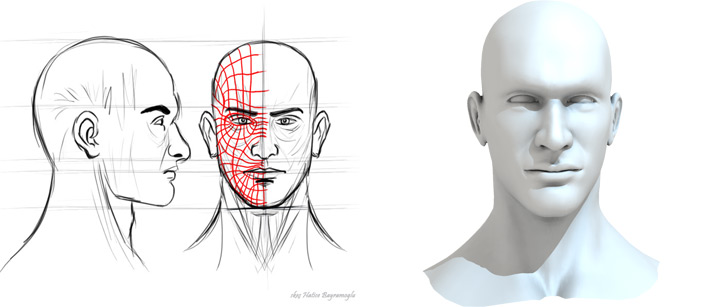
\includegraphics[width=12cm]{images/face-wire.jpg}
\caption{Szkic siatki głowy wraz z modyfikacją profilu~\cite{bayramoglu}}
\end{figure}

Można wyraźnie zauważyć trzy obszary: oko, nos z ustami, ucho. Mając już
oddzielone skomplikowane pod względem szczegółowości obszary, pozostała część
głowy nie jest skomplikowana i gładka więc można ją z powodzeniem zamodelować za
pomocą dosłownie kilku odpowiednio rozciągniętych sfer.

\subsection{Nieterminale w gramatyce kształtu}
Mając podzieloną strukturę głowy na mniejsze obszary należy zamodelować przy
użyciu podstawowych kształtów (łatwych do zapisania matematycznie) wszystkie
poszczególne obszary. Jako kształty łatwe do zapisania matematycznie
przyjęto: sferę, sześcian, płaszczyznę, cylinder, stożek i temu podobne. Za
pomocą tych kształtów oraz ich kombinacji (suma logiczna --- łączenie, różnica
--- wycinanie) można zamodelować dowolną część ludzkiej głowy. Jakość końcowa
wymodelowanej głowy zależy tylko od ilości wykorzystanych podstawowych
kształtów.

Wykorzystanie takich elementów nie będzie wystarczające do zbudowania modelu
więc zdecydowano się na dodanie trzech funkcji przekształcających obiekty:
przesunięcie, obrót i skalowanie. Nic nie stoi na przeszkodzie, żeby rozszerzyć
gramatykę o np. przekształcenia deformujące, takie jak: zwężenie, skręcenie i
wygięcie. Ograniczeniem jest tylko złożoność obliczeniowa danego
przekształcenia.

Kolejną sprawą jest łączenie podstawowych, przekształconych kształtów i do tego
celu wybraliśmy cztery podstawowe operacje Boolowskie: OR (suma logiczna), AND
(część wspólna), DIFF (różnica), XOR (różnica symetryczna). Te przekształcenia
umożliwią nam łączenie, wycinanie i tworzenie skomplikowanych obiektów z
wykorzystaniem dwóch podstawowych kształtów wspomnianych wyżej.

Do zamodelowania wspomnianych wcześniej symetrycznych części głowy należy dodać
funkcję MIRROR --- czyli odbicie lustrzane wymodelowanego już wcześniej
kształtu, względem wybranej płaszczyzny.

Wymienione wyżej podstawowe kształty i przekształcenia są wystarczające do
zamodelowania dowolnej głowy (a nawet całego ciała ludzkiego).

\subsection{Parser gramatyki kształtu}
Do tworzenia gramatyki kształtu zostanie wykorzystany tekstowy zapis kolejnych
operacji. Niezbędny jest również algorytm transformujący język zrozumiały dla
użytkownika programu do formy zrozumiałej przez program. Jako że celem tej pracy
nie jest opracowywanie parsera, zdecydowaliśmy się na wykorzystanie do tego celu
język LUA, ponieważ jest prosty do zaadoptowania do dowolnego projektu.
Korzystając dodatkowo z biblioteki tolua++ sprowadza się to do przygotowania
odpowiednio okomentowanych klas. Skrypt tolua++ parsuje plik nagłówkowy
opisujący klasę jaka ma być dostępna z poziomu skryptu LUA i zwraca plik
źródłowy, który wystarczy dołączyć do projektu.

\subsection{Reprezentacja gramatyki wewnątrz projektu}
Kolejnym ważnym krokiem do zbudowania projektu jest opracowanie struktury
przechowującej gramatykę, zachowując kolejność przetwarzania terminali i
nieterminali. Doskonałą do tego celu strukturą jest drzewo, gdzie liśćmi są
terminale, węzłami są nieterminale stanowiące operacje boolowskie, natomiast
przekształcenia takie jak rotacja, skalowanie i przesunięcie --- metodami
węzłów. Poniżej znajduje się fragment kodu ilustrujący omawianą reprezentację:

{
\small
\begin{lstlisting}[language=C++,numbers=left,frame=single,numberstyle=\tiny,backgroundcolor=\color{code_back},breaklines=true]
class Node
{
    protected:
        typedef boost::shared_ptr<Node> node_ptr;
        typedef const boost::shared_ptr<Node> const_node_ptr;
        typedef boost::weak_ptr<Node> parent_ptr;
        typedef const boost::weak_ptr<Node> const_parent_ptr;
        typedef std::list<node_ptr> t_child_list;

        const_node_ptr _this;
        parent_ptr parent;
        t_child_list childs;

    public:
        Node();
        virtual ~Node();

        bool has_parent();
        bool has_child();
		void attach(node_ptr new_child);
		void attach(node_ptr new_child, t_child_list::iterator it);
		void attach_to(node_ptr p);
		void attach_to(node_ptr p, t_child_list::iterator it);
		t_child_list::iterator detach();
		virtual node_ptr clone();
		virtual node_ptr clone(node_ptr n);
};
\end{lstlisting}
}

Klasa Node jest podstawowym elmentem drzewa, które jest tworzone z gramatyki.
Każdy węzeł może posiadać dowolną liczbę podelementów.

{
\small
\begin{lstlisting}[language=C++,numbers=left,frame=single,numberstyle=\tiny,backgroundcolor=\color{code_back},breaklines=true]
class Nonterminal // tolua_export
: public Node
{ // tolua_export
    protected:
        vl::mat4 tmpMatrix;
        vl::mat4 tmpMatrixInv;
        std::list<vl::mat4> modelMatrix;

    private:
        void buildModelMatrix();

    public:
        vl::mat4 getModelMatrix() const;

    public:
        // tolua_begin
        Nonterminal();
        virtual ~Nonterminal();

        void scale(float x, float y, float z);
        void translate(float x, float y, float z);
        void rotate(float p, float y, float r);
        // tolua_end

        void prepare();
        virtual bool hit(vl::vec4& p, vl::vec4& v, set& s);
        virtual bool hit(vl::vec4& p);
        virtual bool rayTrace(vl::vec4& p, vl::vec4& v, set& s);
        virtual bool rayTrace(vl::vec4& p);
        virtual Node::node_ptr clone();
        virtual Node::node_ptr clone(Node::node_ptr);
}; // tolua_export
\end{lstlisting}
}

Nonterminal jest klasą reprezentującą nieterminal gramatyki kształtu zmapowany
na element drzewa. Klasa pozwala na wykonanie kilku podstawowych transformacji
oraz udostępnia interfejs w postaci kilku metod, które muszą być
zaimplementowane, aby algorytm tworzenia kształtu przebiegał poprawnie:
\begin{itemize}
  \item Nonterminal::hit() -- ma za zadanie zwrócić wartość {\em true}, jeśli
  w wyznaczonym miejscu (określonym przez parametry) znajduje się obiekt. W
  przeciwnym razie metoda powinna zwrócić wartość {\em false}. Metoda ma dwie
  instancje --- z jednym parametrem oraz z trzema. Z jednym parametrem 
  (określającym położenie w przestrzeni $\mathbb{R}^3$) używana jest do
  generowania obiektu w przestrzeni wokselowej, gdyż mamy ustalony na stałe
  jej rozmiar i sprawdzamy woksel po wokselu czy znajduje się tam obiekt. Metoda z trzema parametrami jest
  wykorzystywana do renderowania metodą ray-tracingu (stąd 3 parametry: punkt
  wystrzelenia promienia, wektor promienia oraz zbiór trafień). Algorytm
  ray-tracingu będzie opisany dokładniej w dalszej części pracy;
  \item Nonterminal::rayTrace() -- metoda odpowiedzialna za kolejne etapy
  przeszukań przestrzeni. Podobnie jak w poprzednim przypadku
  posiada dwie instancje: jednoparametrową dla przeszukań w przestrzeni wokselowej i
  trzyparametrową dla przeszukań metodą ray-tracingu.
\end{itemize}

{
\small
\begin{lstlisting}[language=C++,numbers=left,frame=single,numberstyle=\tiny,backgroundcolor=\color{code_back},breaklines=true]
class Sphere : public Nonterminal { // tolua_export
    public:
    // tolua_begin
        Sphere();
        ~Sphere();
    //tolua_end
        virtual bool hit(vl::vec4& p, vl::vec4& v, set& s);
        virtual bool hit(vl::vec4& p);
        virtual Node::node_ptr clone();
}; // tolua_export

class Cylinder : public Nonterminal { // tolua_export
    public:
    // tolua_begin
        Cylinder();
        ~Cylinder();
    //tolua_end
        virtual bool hit(vl::vec4& p, vl::vec4& v, set& s);
        virtual bool hit(vl::vec4& p);
        virtual Node::node_ptr clone();
    private:
        float r;
        float h;
        vl::vec3 rdir;
        vl::vec3 hdir;
        vl::vec3 center;
}; // tolua_export

class And : public Nonterminal { // tolua_export
    public:
        And() {}
    // tolua_begin
        And(Nonterminal& t1, Nonterminal& t2);
        And(Nonterminal& t1, Nonterminal& t2, Nonterminal& t3);
        And(Nonterminal& t1, Nonterminal& t2, Nonterminal& t3, Nonterminal& t4);
        And(Nonterminal& t1, Nonterminal& t2, Nonterminal& t3, Nonterminal& t4, Nonterminal& t5);
        ~And();
    //tolua_end
        virtual bool rayTrace(vl::vec4& p, vl::vec4& v, set& s);
        virtual bool rayTrace(vl::vec4& p);
        virtual Node::node_ptr clone();
}; // tolua_export

class Or : public Nonterminal { // tolua_export
    public:
        Or() {}
    // tolua_begin
        Or(Nonterminal& t1, Nonterminal& t2);
        Or(Nonterminal& t1, Nonterminal& t2, Nonterminal& t3);
        Or(Nonterminal& t1, Nonterminal& t2, Nonterminal& t3, Nonterminal& t4);
        Or(Nonterminal& t1, Nonterminal& t2, Nonterminal& t3, Nonterminal& t4, Nonterminal& t5);
        ~Or();
    //tolua_end
        virtual bool rayTrace(vl::vec4& p, vl::vec4& v, set& s);
        virtual bool rayTrace(vl::vec4& p);
        virtual Node::node_ptr clone();
}; // tolua_export

class Diff : public Nonterminal { // tolua_export
    public:
        Diff() {}
    // tolua_begin
        Diff(Nonterminal& t1, Nonterminal& t2);
        Diff(Nonterminal& t1, Nonterminal& t2, Nonterminal& t3);
        Diff(Nonterminal& t1, Nonterminal& t2, Nonterminal& t3, Nonterminal& t4);
        Diff(Nonterminal& t1, Nonterminal& t2, Nonterminal& t3, Nonterminal& t4, Nonterminal& t5);
        ~Diff();
    //tolua_end
        virtual bool rayTrace(vl::vec4& p, vl::vec4& v, set& s);
        virtual bool rayTrace(vl::vec4& p);
        virtual Node::node_ptr clone();
}; // tolua_export

class Xor : public Nonterminal { // tolua_export
    public:
        Xor() {}
    // tolua_begin
        Xor(Nonterminal& f, Nonterminal& s);
        ~Xor();
    //tolua_end
        virtual bool rayTrace(vl::vec4& p, vl::vec4& v, set& s);
        virtual bool rayTrace(vl::vec4& p);
        virtual Node::node_ptr clone();
}; // tolua_export

class Mirror : public Nonterminal { // tolua_export
    public:
        Mirror() {}
    // tolua_begin
        Mirror(Nonterminal& t, char type);
        ~Mirror();
    //tolua_end
        virtual Node::node_ptr clone();
}; // tolua_export
\end{lstlisting}
}

Klasy Sphere oraz Cylinder to operatory tworzące kształty (ang.
brush\footnote{W terminologi grafiki komputerowej pojęcie to jest używane w
celu określenia obiektu o pewnym kształcie, który służy do tworzenia bądź
modyfikacji istniejącego modelu. Pędzle wykorzystywane są m.in. w programie
Sculptris, ZBrush do ,,rzeźbienia'' obiektów}.) odpowiednio sfery oraz cylindra.
Aby uzyskać odpowiedni rozmiar, pozycję oraz orientację należy wykorzystać
metory scale, transtale i rotate.
Na kształtach zdefiniowanych przez operatory Sphere i Cylinder można wykonywać
różne operacje logiczne oraz tworzyć lustrzane odbicia. Te funkcjonalności
zaimplementowane są przez klasy And, Or, Diff, Xor i Mirror.
